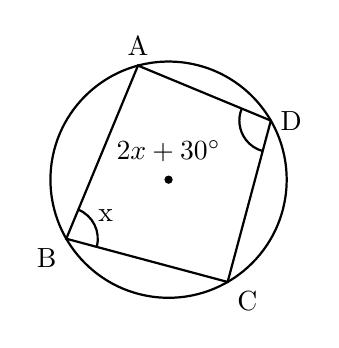
\begin{tikzpicture}[scale=1]

  % Define the center of the circle
  \coordinate (O) at (0,0);

  % Define the radius of the circle
  \def\R{1.5}

  % Draw the circle
  \draw[thick] (O) circle (\R);

  % Add a dot at the center
  \fill (O) circle (1.5pt);

  % Define the points A, B, C, D on the circle
  % A is top-ish
  \coordinate (A) at (105:\R);
  % B is bottom-left
  \coordinate (B) at (210:\R);
  % C is bottom-right
  \coordinate (C) at (300:\R);
  % D is top-right
  \coordinate (D) at (30:\R);

  % Draw the quadrilateral ABCD
  \draw[thick] (A) -- (B) -- (C) -- (D) -- cycle;

  % Draw the angle arc at B (angle x)
  % Angle from BC (-15°) to BA (67.5°)
  \draw[thick] (B) +(-15:0.4) arc (-15:67.5:0.4);
  \node at (-0.8, -0.45) {x};

  % Draw the angle arc at D
  % Angle from DA (157.5°) to DC (255°)
  \draw[thick] (D) +(157.5:0.4) arc (157.5:255:0.4);

  % Add the label for angle 2x+30° near the center
  \node[above] at (0,0.1) {$2x+30^\circ$};

  % Add labels for the vertices
  \node[above] at (A) {A};
  \node[below left] at (B) {B};
  \node[below right] at (C) {C};
  \node[right] at (D) {D};

\end{tikzpicture}